
\documentclass[11pt]{article}
\usepackage[font=small,labelfont=bf]{caption}
\usepackage{graphicx}
\usepackage{amsmath}
\usepackage{hyperref}\usepackage{color}
\usepackage{parskip}
\usepackage{float}
\usepackage{tabularx}
\usepackage{appendix}
\usepackage{rotating} \usepackage{verbatim} \usepackage{lscape}
\usepackage{dcolumn} \usepackage{ctable} \usepackage{amssymb}
\usepackage{longtable}
\usepackage{threeparttable}
\usepackage{pdflscape}
\usepackage{cases}
 \usepackage[ style=authoryear,backend=biber, url=true]{biblatex}
 \addbibresource{proposal.bib}

\title{Exporting/Importing and firm performance: Evidence from India}
\author{Arjun Gupta}
%\institution{National Institute of Public Finance and Policy}
\newcommand{\alert}[1]{#1}

\newcommand{\floatintro}[1]{
  
  \vspace*{0.1in}
  
  {\footnotesize
    
    #1
    
  }
  
  \vspace*{0.01in}
}
%Introduce floatintros
\definecolor{red}{rgb}{0.0,0.0,0.0}
\hypersetup{colorlinks,breaklinks,linkcolor=red,urlcolor=red,anchorcolor=red,citecolor=red}
\floatstyle{ruled} 
\restylefloat{table} 
\restylefloat{figure}

\begin{document}
\maketitle


\begin{abstract}
 
\end{abstract}


\newpage
\small

\tableofcontents

\newpage
\section{Introduction}\label{sec:introduction}



There is vast literature  which states that exporters tend to
out-perform non-exporters in terms of wages, capital,
productivity. \cite{bernard1999exceptional}  say that this can be due
to these reasons:
\begin{itemize}
\item export increases productivity (Self-selection)
\item productivity increases export (Learning by doing)
\end{itemize}

Self-selection (SS) hypothesis  of more productive firms into export states that 
participation in the export market is accompanied by additional costs
such as transport costs, establishing a distribution channel,
cost of traversing beaurocratic channles  etc. This means that there
are substantial sunk costs to participating in the export market. Therefore, firms which are more productive plan to
enter to the export market. 

Learning-by-doing hypothesis (\cite{haidar2012trade}) states that exporting firms deal with
tougher competition in the international market as compared to the
domestic market, and therefore must improve their performance to
remain active in the export market. Moreover, participating in the
international market leads knowledge flows from international buyers
to help post entry performance of export starters. This means that exporting should
cause productivity spillovers as well.

The same hypothesis (self-selection and learning-by-doing) can  apply
to import behavior of firms. Since importing also involves additional
similar costs like additional taxes, transport costs etc. , firms that
are more productive will enter the import market. Also, a firm
participating in the import market can have access to better
technology and higher quality goods. \cite{topalova2011trade}  and \cite{halpern2011imported}
find that improved access to foreign technology can boost
productivity. 

Since, participating in the export/import market  could involve costs that
are complimentary. It would be interesting to see how participation in
one activity affects the other.  I plan to investigate is whether there
are benefits of importing to exporting and vice-versa by estimating
the complementary nature between the two. 


So, my reasearch plan is to investigate:
\begin{itemize}
\item Self-selection hypothesis: Check whether more productive firms
  participate in the expprt/import market
\item Learning-by-doing hypothesis: Check if there are productivity
  spillovers from participation in the export/import market
\item Estimate the fixed and sunk costs of participation in the
  export/import market and the decrease in costs due to the
  complimentary nature between the two
\item Run counter-factual experiment to see the effect of decrease in
  the costs to exporting/importing. 
\end{itemize}




\section{Data}\label{sec:data}
I use annual firm level data from Centre for Monitoring Indian Economy
(CMIE) which provides  data from 1989 to 2017. 

I fetch the following variables from CMIE: 

\begin{center}
\input{./TABLES/indicatordescription.gen}
\end{center}

Table 1 shows the variables and their meaning. I chose the variables
which might be the most pertinent to my research question. 

The variables stated above are nominal values. I fetch Wholseale Price
Index (WPI), which provides the inflation rate of the wholesale prices
and deflate the variables to give real values. Then, I clean the data
to remove missing values and select firms with the broad industry
classification code indicating that they are a manufacturing
firms to get the following composition of firms: 
\begin{center}
\input{./TABLES/compnfirms.gen}
\end{center}
India liberalised its economy in 1992 which resulted in import
tariffs, deregulation of markets, reduction of taxes, and greater 
foreign investment. According to \cite{topalova2011trade}, The government's trade policy under the Eighth Five�]Year Plan (1992-97) ushered
in radical changes to the trade regime by sharply reducing the role of
the import and export control system. The share of products subject to quantitative restrictions
decreased from 87 percent in 1987�]88 to 45 percent in 1994-95, and the actual user
condition on imports was discontinued. And since 1997, the decrease in
output and input tariff has been very marginal. Therefore I restrict
the time period of the study from 1997 to 2016.  Since, firms
are under no legal obligation to report their finances, which might
mean that mean that small firms are less likely to report their
finances. However, this dataset includes all publicly listed firms as
their firm financials are public information. This might affect my
results as it is biased towards bigger firms. 

I create two additional variables \textit{Export} , \textit{Import},
\textit{Domestic Sales}
by adding the following variables from the Table 1.  
\begin{enumerate}
\item Export: sa\_export\_goods $+$ sa\_export\_serv
\item Import: sa\_import\_rawmat $+$        sa\_import\_stores\_spares
  $+$ sa\_import\_fg            $+$sa\_import\_cap\_goods
\item Domestic Sales: Total Sales - Export Sales
\end{enumerate}
Then, I create four dummy variables of trade market participation
using the \textit{Export} and \textit{Import} variables: 
\begin{itemize}
\item None: Firms that do not participate in the export/import market
\item Export only: Firms that participate in the export market only
\item Import only: Firms that participate in the import market only
\item Both: Firms that participate in both export/import market
\end{itemize}
Table 3 displays the composition of firms according to their trade market
participation status. It is seen that number of firms that do not
participate in the trade market is low,  around 20 to 35
\%. Surprisingly, the number of firms that participate in the trade
market is really high. Another interesting feature is that the number
of firms that participate only in the import market is higher than the
firms that participate only in the export market. This must mean that
the demand for foreign intermediaries is really high. Almost 50 \% of
firms in each year participate in both export/import market.  It is
also seen that the participation rate in the trade is not increasing
year on year.  
\begin{center}
\input{./TABLES/composition.gen}
\end{center}
\section{Descriptive Statistics}
\subsection{Self-Selection}
As a first step to see if more productive firms self-select into
participating in the trade market, I calculated the mean and standard
deviation and created the density plots for log of  sales, gross fixed assets,
salaries and  expenditure on power and fuel. 
Tables 4-6 and 10-12 display the results for the variables mentioned above. 
It can be seen that firms that participate in the trade market have
higher mean for all the variables mentioned above. It is also seen
that firms that participate in the both export/import market have
higher mean of sales,gross fixed assets,
salaries, expenditure on power and fuel than firms that participate in
only export and only import. On the other hand, the standard deviation in all
the cases is very similar. 



\begin{center}
\begin{table}[tp]
\caption{Summary statistics of Sales (log)}
\begin{tabular}{c}
 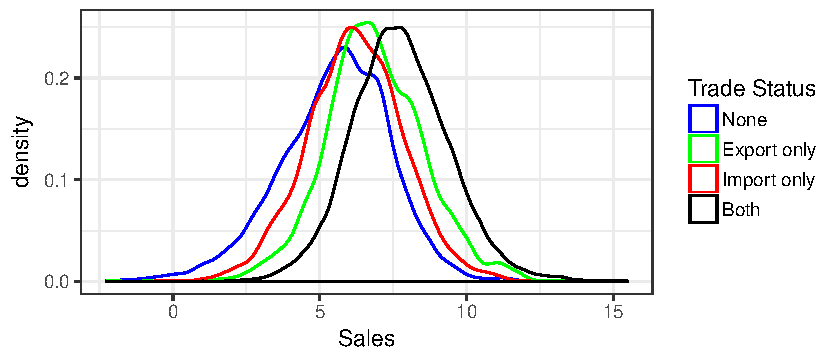
\includegraphics{./PICS/denslsales.pdf}   \\ 
 \input{./TABLES/sumstatslsales.gen}  \\  
\end{tabular}
\end{table}
\end{center}

\begin{center}
\begin{table}[tp]
\caption{Summary statistics of Gross Fixed Assets (log)}
\begin{tabular}{c}
 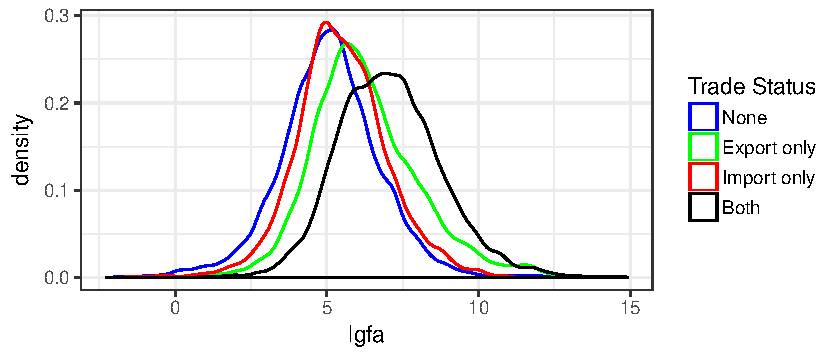
\includegraphics{./PICS/denslgfa.pdf}   \\ 
 \input{./TABLES/sumstatslgfa.gen}  \\  
\end{tabular}
\end{table}
\end{center}

\subsection{Complementarity between Exporting and Importing}
Table 9 displays the export value for firms that participate only in the
export market and for firms that participate in both export/import
market. 
It is seen in Table 9 that firms that participate in both the
export/import market have a higher exports than firms that only
participate in the export market. This suggests that importing has a
positive effect on exporting.   
\begin{center}
\begin{table}[tp]
\caption{Summary statistics of Export (log)}
\begin{tabular}{c}
 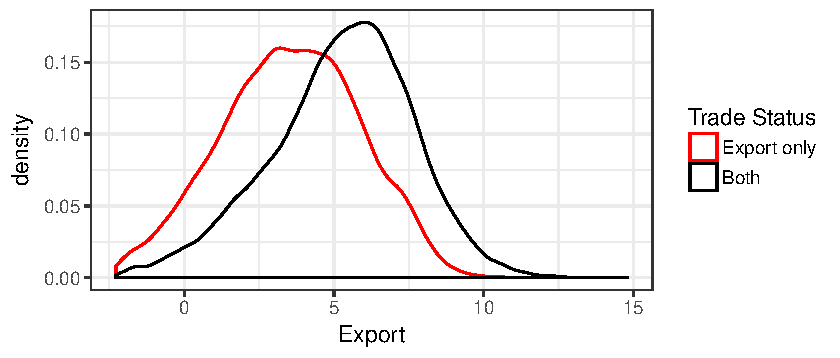
\includegraphics{./PICS/denslexport.pdf}   \\ 
 \input{./TABLES/sumstatslexport.gen}  \\  
\end{tabular}
\end{table}
\end{center}
Table 10 displays the import value for firms that participate only in the
import market and for firms that participate in both export/import
market. 
It is seen in Table 10 that firms that participate in both the
export/import market have a higher imports than firms that only
participate in the import market. This suggests that exporting has a
positive effect on importing.  

\begin{center}
\begin{table}[tp]
\caption{Summary statistics of Import (log)}
\begin{tabular}{c}
 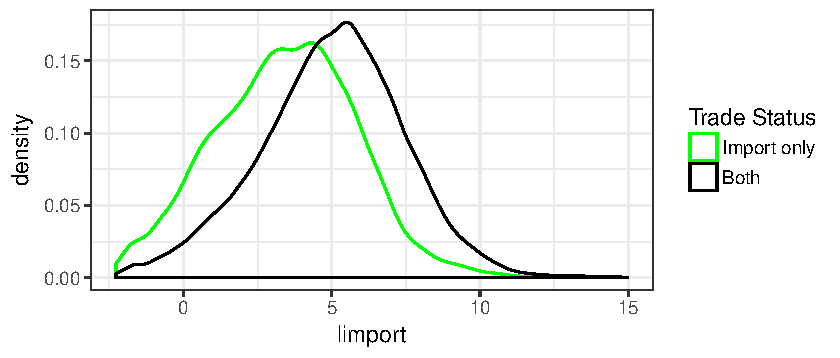
\includegraphics{./PICS/denslimport.pdf}   \\ 
 \input{./TABLES/sumstatslimport.gen}  \\  
\end{tabular}
\end{table}
\end{center}
Table 6 and Table 7 suggest that both these activities have a
positive effect on the other and This might be because importing
complements exporting and vice-versa. Therefore, there is correlation between these
activities that needs further research. 

% \begin{center}
% \input{./TABLES/transition.gen}
% \end{center}


\subsection{Productivity and Export/Import}
\cite{gupta2018exporting} define a rough measure of productivity known
as \textit{capital productivity}. It is defined as the log of value added per
unit of capital used by a firm:

$$ log(VA_{it} - log(K_{it})$$
where $VA_{it}$ is firm-level value added, computed as total industrial sales plus
change in stock minus power and fuel expenditures, and raw material
expenses. Table * displays the summary statistics for this variable
based on the trade activity status. It can be seen that mean of capital
productivity increases as activity status moves from \textit{None} to
\textit{Export only/Import only} to \textit{Both}, whereas the
standard deviation also decreases.  
\begin{center}
\begin{table}[tp]
\caption{Summary statistics of Capital Productivity (log)}
\begin{tabular}{c}
 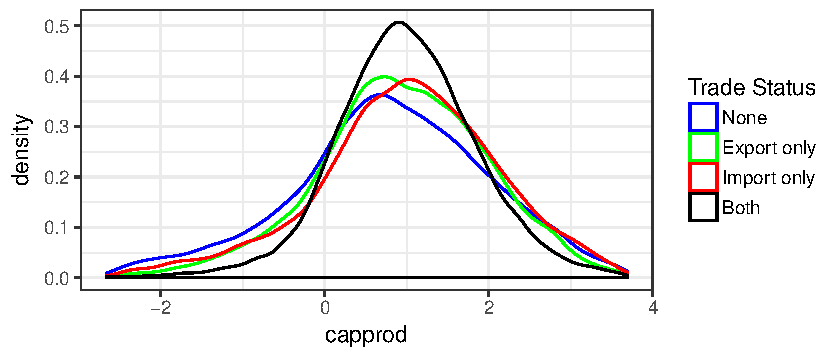
\includegraphics{./PICS/denscapprod.pdf}   \\ 
 \input{./TABLES/sumstatscapprod.gen}  \\  
\end{tabular}
\end{table}
\end{center}

Table 12 displays the summary statistics of Profit to Sales based on a
firms trade market status. Profit to sales is calculated by dividing
the profit after tax with sales. This measure can be interpreted as a
profitability measure. It is seen in table 12 that participating in
the trade market increases the profit to sales ratio. Firms that do
not participate in the trade market have a very high standard
deviation of profit to sales. It is also interesting to see that mean
profit to sales ratio in every case is negative. 
\begin{center}
\begin{table}[tp]
\caption{Summary statistics of Profit to Sales}
\begin{tabular}{c}
 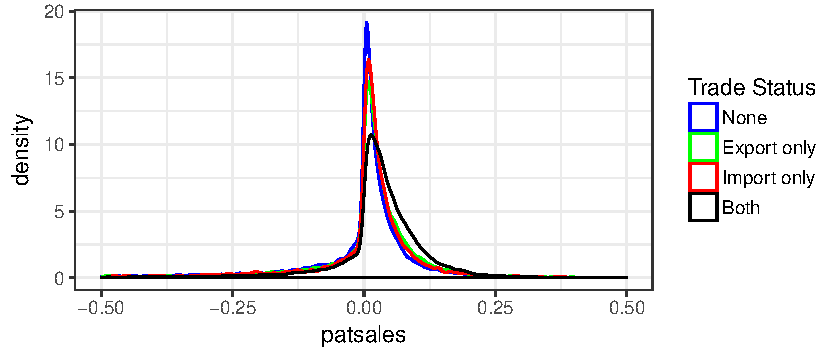
\includegraphics{./PICS/denspatsales.pdf}   \\ 
 \input{./TABLES/sumstatspatsales.gen}  \\  
\end{tabular}
\end{table}
\end{center}



\section{Model}

I use a model inspired from  \cite{aw2011}, \cite{de2011product} and \cite{kasahara2013productivity}. 

\subsection{Static Decision}

A firm i has a standard Cobb-Douglas Production Function 

\begin{equation}
Q_{it} =
k_{it}^{\alpha_k}L_{it}^{\alpha_l}M_{it}^{\alpha_m}exp(\omega_{it} + u_{it})
\end{equation}
where 
\begin{itemize}
\item $K_{it}$ is the unit of output
\item $L_{it}$ is the unit labour
\item $M_{it}$ is the domestic and imported unit of materials
\item $\omega_{it}$ is the productivity shock
\item $u_{it}$ is the measurement error
\end{itemize}

A firm faces a constant elasticity of demand (CES) function assumed to
be of the Dixit-Stiglitz form :

\begin{equation}
Q_{it}^{D} = Q_{dt}(\frac{P_{it}}{P_{dt}})^{\eta_{d}}
\end{equation} 
where $Q_{idt}^{d}$ is the industry aggregate output, $P_{dt}^{d}$ is
the price index and $P_{it}^{d}$ is the firm i's price. 

The demand function in the export market has a similar structure
except that it also depends on an industry-specific demand shifter: 
\begin{equation}
Q_{it}^{X} = Q_{Xt}(\frac{P_{it}^{X}}{P_{dt}^{X}})^{\eta_{X}}exp(z_{it})
\end{equation} 
where $z_{it}$ is the unobserved firm specific demand
shock. 

Equation 2 can be used to obtain an expression for $P_{it}$ and a
firms domestic revenue is $R_{it} = P_{it}Q_{it}$, and inserting price
into the revenue function and taking a log to get the revenue function
in the domestic market:

\begin{equation}
\tilde{r_{it}} = \beta_{l}l_{it} + \beta_{m}M_{it} + \beta_{K}K_{it} +
\beta_{d}Q_{dt} + \omega^{*}_{it} + u_{it}
\end{equation}
 The revenue function for the export market can be similarly derived
 to get:
\begin{equation}
\tilde{r_{it}} = \beta_{l}l_{it} + \beta_{m}M_{it} + \beta_{K}K_{it} +
\beta_{X}Q_{Xt} + \omega^{*}_{it} + u_{it} + z^{*}_{it}
\end{equation}
where $\beta_{h}= \frac{\eta_{d}+1}{\eta_{d}}\alpha_{h}$, $\beta_{s.m} =
\frac{1}{\eta_{d}}$, $\omega^{*}_{it} =
\omega^{*}_{it}\frac{\eta_{d}+1}{\eta_{d}}$ and $z^{*}_{it} =
z_{it} eta_{d}^{-1}$


\cite{das2007market} display a relation between profits and revenue. I
use this estimate the constant demand of elasticity in both the
domestic and export market. 
In the domestic market, the profits are: 
\begin{equation}
\pi_{it}^d = \frac{1}{\eta_{d}} r_{it}^{d}(K_{it}, \omega_{it})
\end{equation} 

In the export market, the profits are: 
\begin{equation}
\pi_{it}^X = \frac{1}{\eta_{X}} r_{it}^{X}(K_{it}, \omega_{it})
\end{equation} 

\subsection{Transition of Productivity}

The firm-level productivity is allowed to the be endogenously affected
by the firms decision to export and import. Therefore, the law of
motion of productivity is:

\begin{equation}
\omega_{it} = g(\omega_{it-1}, d_{it-1}^{X}, d_{it-1}^{M}) + \nu_{it}
\end{equation}

\begin{equation}
\omega_{it} = \alpha_{o} + \alpha_{1}\omega_{it-1} +
\alpha_{2}\omega_{it-1} + \alpha_{3}\omega_{it-1}^{2}+
\alpha_{4}d_{it-1}^{X} + \alpha_{5} d_{it-1}^{M} + \alpha_{6}d_{it-1}^{X}d_{it-1}^{M}  \nu_{it}
\end{equation}

where $d_{it-1}^{X}$ is an indicator function of the firms lagged export
participation, $d_{it-1}^{M}$ is an indicator function of the firms lagged import
participation and $\nu_{it}$ is an iid shock to the productivity. The
lagged export and import indicator variables allow for
learning-by-exporting and productivity benefits from importing. 

The model assumes that productivity is only affected by the intensity
of export/importing but is only dependent on the decision. 

The firm-specific demand shock is modelled as an AR(1) process. 



\subsection{Dynamic Model}
 
Firm must pay a fixed/sunk costs of trading. Let $d_{i,t}^X$ be the
indicator function of participation in the export market and
$d_{i,t}^M$ be the indicator function of participation in the import
market. Then the total costs paid by firm i in period t is given by:


$F(d_{it}, d_{it-1})= $
\begin{enumerate}
\item   $f^{x} + c^{X}(1 - d_{it-1}^X)$\hfill  for $ (d_{it}^X, d_{it}^M) =
  (1,0) $
\item   $f^{x} + c^{M}(1 - d_{it-1}^M)$\hfill  for $ (d_{it}^X, d_{it}^M) =
  (0,1) $
\item   $\lambda[f^{x} + f^{M} + c^{X}(1 - d_{it-1}^X) + c^{M}(1 -
  d_{it-1}^M)]$  \hfill for $ (d_{it}^X, d_{it}^M) =
  (1,1) $
\item   0  \hfill for $ (d_{it}^X, d_{it}^M) =
  (0,0) $
\end{enumerate}
Here $f^{X}$ is the fixed cost of exporting,$C^{X}$ is the sunk cost
of exporting, $f^{M}$ is the fixed cost of importing, $f^{M}$ is the
fixed cost of importing and $\lambda$ captures the degrees of
complementarity between exporting and importing. 

$$ S_{it} = (\omega_{it}, K_{it}, d_{it-1}^{X}, d_{it-1}^{M})$$

\begin{equation}
V_{it}(S_{it}) = max_d(\pi_{it}^{d} +d_{it}\pi_{it}^{X} + F(d_{it}, d_{it-1}) + \beta E(V_{it}(s_{it+1}|s_{it})))
\end{equation}

% Therefore, for any state vector, the marginal benefit of exporting is
% equal to:

% \begin{equation}
% MBE(S_{it}|d_{it-1}) = \pi_{it}^X + V_{it}(s_{it}|e_{it-1}=1) - V_{it}(s_{it}|e_{it-1}=0)
% \end{equation}

% Therefore, for any state vector, the marginal benefit of importing is
% equal to:

% \begin{equation}
% MBM(S_{it}|d_{it-1}) =  V_{it}(s_{it}|M_{it-1}=1) - V_{it}(s_{it}|M_{it-1}=0)
% \end{equation}

% \begin{equation}
%   V_{it}(s_{it}) = \int (\pi_{it}^D + max_{e_{it}}\{( \pi_{it}^D +
%   e_{it-1}\gamma_{it}^{F} - (1- e_{it})\gamma_{it}^{S}) + V_{it}^{E}(s_{it}) ,
%   V_{it}^{D}(s_{it})\}) dG^{\gamma}
% \end{equation}

 
% \begin{equation}
%   V_{it}(s_{it}) = \int (\pi_{it}^D + max_{e_{it}}\{( \pi_{it}^D +
%   e_{it-1}\gamma_{it}^{F} - (1- e_{it})\gamma_{it}^{S}) + V_{it}^{E}(s_{it}) ,
%   V_{it}^{D}(s_{it})\}) dG^{\gamma}
% \end{equation}


% \begin{equation}
%   V_{it}^E(s_{it}) = \int ( max_{m_{it}}\{ \beta E_{t}
%   V_{it+1}(s_{it+1}|e_{it}=1, m_{it} =1) - m_{it-1} \gamma_{it}^{mf} , \beta E_{t}
%   V_{it+1}(s_{it+1}|e_{it=1}=1, m_{it} =0) \} dG^{\gamma}
% \end{equation}


% \begin{equation}
%   V_{it}^D(s_{it}) = \int ( max_{m_{it}}\{ \beta E_{t}
%   V_{it+1}(s_{it+1}|e_{it}=0, m_{it} =1) - m_{it-1} \gamma_{it}^{mf} , \beta E_{t}
%   V_{it+1}(s_{it+1}|e_{it}=0, m_{it} =0) \} dG^{\gamma}
% \end{equation}
\section{Estimation}
\printbibliography[omitnumbers=false]
\section{Appendix}
\subsection{Descriptive Statistics}
\begin{center}
\begin{table}[tp]
\caption{Summary statistics of Salary (log)}
\begin{tabular}{c}
 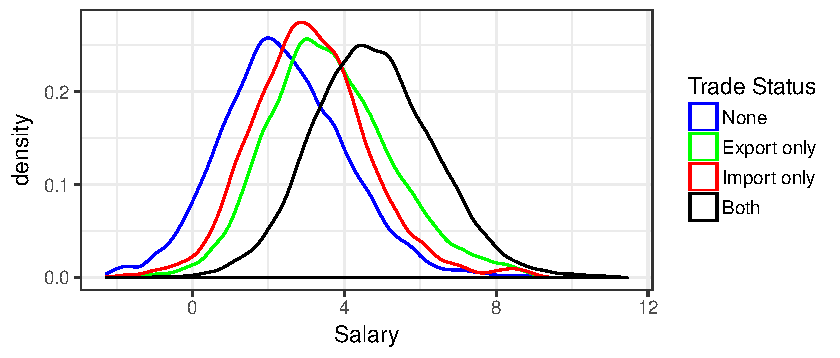
\includegraphics{./PICS/denslsalary.pdf}   \\ 
 \input{./TABLES/sumstatslsalary.gen}  \\  
\end{tabular}
\end{table}
\end{center}

\begin{center}
\begin{table}[tp]
\caption{Summary statistics of Expenditure on raw material (log)}
\begin{tabular}{c}
 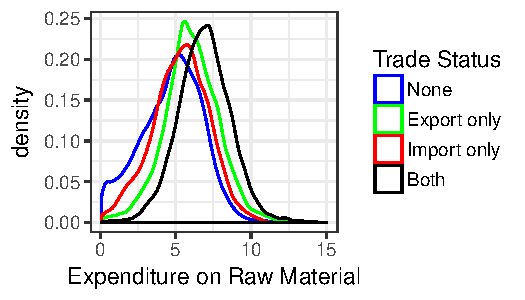
\includegraphics{./PICS/denslrawmat.pdf}   \\ 
 \input{./TABLES/sumstatslrawmat.gen}  \\  
\end{tabular}
\end{table}
\end{center}

\begin{center}
\begin{table}[tp]
\caption{Summary statistics of expenditure on power and fuel (log)}
\begin{tabular}{c}
 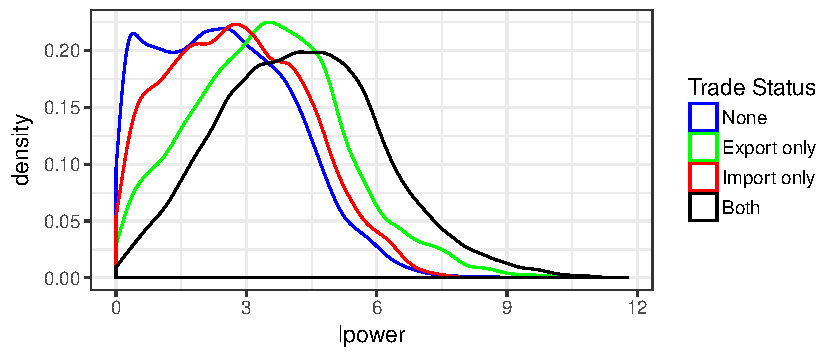
\includegraphics{./PICS/denslpower.pdf}   \\ 
 \input{./TABLES/sumstatslpower.gen}  \\  
\end{tabular}
\end{table}
\end{center}

\subsection{Productivity Estimation}
\subsubsection{Levinsohn-Petrin Productivity Estimation}
\cite{levinsohn2003estimating} suggest a strategy to estimate
productivity and it goes as follows:

Let the production function be: 
\begin{equation}
y_{it} = \beta_{o} + \beta_{l}l_{it} + \beta_{k}K_{it} +\beta_{I}I_{it}+ \omega_{it} + \eta_{it} 
\end{equation}
where $l_[it}$ is labour, $K_{it}$ is capital, $I_{it}$  is
intermediate input, $\omega_{it}$ is firm-level-productivity
observable to the firm and $\eta_{it}$ is an iid shock.\\

Here, the intermediated input demand function is given by:
$$  I_{it} = I_{it}(\omega_{it}, k_{it})$$
This function is assumed to be montonically increasing and therefore
productivity can be found by inverting the function above. Therefore,
we can write the equation above as: 
$$ y_{it} = \beta_{l}l_{it} + \phi_{it}(I_{it},K_{it})$$
where $\phi_{it}(I_{it},K_{it}) = \beta_{o} + \beta_{k}K_{it}
+\beta_{I}I_{it}+ \omega_{it}(I_{it}, K_{it})$

Therefore, 

$$ y_{it}^{*} = y_{it} - \beta_{l}l_{it} = \beta_{o} + \beta_{k}K_{it}
+\beta_{I}I_{it}+ \omega_{it}(I_{it}, K_{it})$$
 
It is also assumed that $\omega_{it}$ follows a first order markov
process : 
$$\omega_{it} = E[\omega_{it}|\omega_{it-1}] + \epsilon_{it}$$ 
Therefore, the equation above can be written as: 

\begin{equation}
y_{it}^{*} = \beta_{o} + \beta_{k}K_{it}
+\beta_{I}I_{it}+ E[\omega_{it}|\omega_{it-1}] + \epsilon_{it}
\end{equation}

\end{document}

